\documentclass{article}
\usepackage[utf8]{inputenc}
\usepackage[T1]{fontenc}
\usepackage[portuguese]{babel}

\usepackage{indentfirst}
\usepackage{makeidx}
\usepackage{stackengine}
\usepackage{amssymb}
\usepackage{amsthm}
\usepackage{hyperref}
\usepackage{color}
\usepackage{graphicx}

\usepackage{booktabs}

\title{\bf{Aprendizagem Computacional - Trabalho Prático 2}\vspace{80mm}}
\author{\textbf{João Tiago Márcia do Nascimento Fernandes - 2011162899} \\
\textbf{Joaquim Pedro Bento Gonçalves Pratas Leitão - 2011150072}}
\makeindex

\begin{document}

\maketitle

\pagebreak

\renewcommand*\contentsname{Índice}
\tableofcontents

\pagebreak

\section{Introdução}

Este trabalho foca-se no reconhecimento de caracteres da numeração árabe, ou seja, os caracteres 0 a 9.

Pretende-se que este reconhecimento seja realizado por uma aplicação desenvolvida em \emph{Matlab}, que faz uso de redes neuronais na sua arquitetura interna, disponíveis na \emph{Nerual Networks Toolbox} do próprio \emph{Matlab}.

A aplicação desenvolvida visa o estudo de duas arquiteturas distintas no reconhecimento dos caracteres:

\begin{itemize}
\item Na primeira arquitetura a aplicação será constituída por uma \emph{memória associativa} e um \emph{classificador}

\item Na segunda arquitetura a aplicação apenas recorre ao \emph{classificador}
\end{itemize}

\vspace{.3cm}

As duas arquiteturas apresentadas estão presentes nas figuras que se seguem:

\begin{figure}[h]
  \centering
      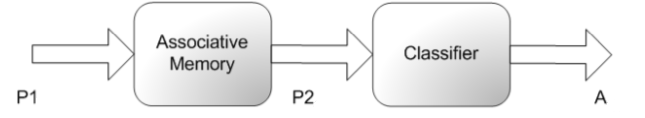
\includegraphics[scale=0.4]{AM_Classifier.png}
  \caption{Arquitetura da aplicação com \emph{memória associativa + classificador}}
\end{figure}

\begin{figure}[h]
  \centering
      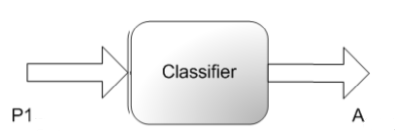
\includegraphics[scale=0.4]{Classifier.png}
  \caption{Arquitetura da aplicação apenas com o \emph{classificador}}
\end{figure}

Através da análise destas figuras podemos determinar um comportamento padrão para a aplicação:

\begin{itemize}
\item Numa fase inicial, os caracteres a identificar poderão, ou não, ser fornecidos à \emph{memória associativa}, que está encarregue da sua "filtragem" ou "correção": Se os caracteres fornecidos não forem perfeitos, a memória associativa aproxima-os dos respetivos caracteres perfeitos.

\item De seguida os dados, corrigidos ou não, serão fornecidos ao \emph{classificador}, que se encarregará de proceder à identificação dos mesmos.
\end{itemize}

No presente documento iremos proceder à apresentação em maior detalhe destas duas arquiteturas e das suas implementações, bem como da aplicação \emph{Matlab} desenvolvida, e de como poderá ser utilizada. Pretendemos também fazer uma análise crítica da performance da aplicação, nomeadamente da sua capacidade de classificar corretamente novos caracteres fornecidos.

\pagebreak

\section{Aplicação Desenvolvida}

A aplicação desenvolvida visa identificar e classificar corretamente caracteres desenhados pelo utilizador, implementando para isso as duas arquiteturas apresentadas anteriormente: \emph{Memória Associativa + Classificador} e \emph{Classificador}.

Esta classificação é realizada atribuindo a cada elemento do conjunto de dados de entrada da aplicação uma \emph{classe}, representada por um número inteiro entre \emph{1} e \emph{10}. Quando um dado elemento é classificado com a \emph{classe 1} então a aplicação indica que o elemento em questão corresponde à escrita manual do número {1}, mantendo-se o raciocínio para as restantes \emph{classes}, com a exceção da \emph{classe 10}, que representa o número \emph{0}.

Ambas as arquiteturas e os respetivos modos de funcionamento serão apresentados de seguida.

\subsection{Memória Associativa + Classificador}

Na arquitetura \emph{Memória Associativa + Classificador}, os caracteres desenhados pelo utilizador, que constituem o \emph{input} da nossa aplicação, são fornecidos à \emph{memória associativa}, onde são \emph{"purificados"}.

Com esta operação pretende-se aproximar os caracteres desenhados pelo utilizador, que são naturalmente imperfeitos, dos respetivos caracteres perfeitamente desenhados. Ao purificarmos os dados estaríamos a aumentar a sua precisão, o que, teoricamente, resultará numa melhor classificação por parte do \emph{classificador}.

Por seu turno, o \emph{classificador} recebe como entradas os caracteres purificados e, com recurso a uma rede neuronal previamente treinada, processa cada uma das suas entradas, produzindo uma classificação para cada uma delas, que corresponde à identificação do caracter em questão, classificação essa que será apresentada ao utilizador.

\subsection{Classificador}

Ao contrário da arquitetura anterior, na arquitetura \emph{Memória Associativa + Classificador}, os caracteres desenhados pelo utilizador não sofrem qualquer tipo de purificação, sendo fornecidos ao \emph{classificador} tal como foram desenhados pelo utilizador.

Tal como o descrito na arquitetura anterior, o classificador recorre a uma rede neuronal previamente treinada para realizar a classificação das entradas. Uma vez classificadas as entradas, o resultado da sua classificação é apresentado ao utilizador.


\subsection{Implementação em Matlab}

Para o desenvolvimento da aplicação foi-nos fornecido código-fonte, que cria e disponibiliza ao utilizador uma grelha onde este irá desenhar os caracteres a identificar, encarregando-se de toda a lógica interna da aplicação com a exceção da implementação do sistema de classificação dos caracteres e de toda a lógica a ele inerente (implementação das diferentes arquiteturas da aplicação, realização dos treinos das redes neuronais implementadas, etc)

\subsubsection{associativeMemory.m}

Neste ficheiro encontra-se uma pequena implementação da memória associativa, presente na função \emph{associativeMemory}. Esta implementção visa \emph{"purificar"} os caracteres desenhados pelo utilizador, aproximando-os do respetivo caracter perfeitamente desenhado. Nesta implementação apenas são calculados os pesos da rede neuronal que constituí a \emph{memória associativa}.

O cálculo dos pesos é feito de duas formas diferentes, com dois conjuntos de dado de treino de diferentes dimensões, escolhidos pelo utilizador. Para o efeito, foram utilizados dados de treino com 100 e 500 casos de teste.

Assim, numa situação, os pesos são calculados recorrendo à fórmula: $target\times input^T$. Na segunda situação, os pesos são calculados de acordo com: $target\times pinv(input)$, onde \emph{input} corresponde aos dados de treino fornecidos à \emph{memória associativa}, \emph{target} corresponde aos respetivos valores esperados à saída da \emph{memória associativa} e \emph{pinv} é uma função específica do \emph{Matlab}.

Uma vez calculados os valores desses pesos a função \emph{associativeMemory} retorna, devolvendo os valores calculados. A \emph{"purificação"} dos dados criados pelo utilizador só será realizada na função \emph{myclassify} (presente no ficheiro \emph{myclassify}), após terem sido obtidos os pesos da \emph{memória associativa}.

\subsubsection{createNetwork.m}

No ficheiro \emph{createNetwork.m} encontramos a função \emph{createNetwork}, responsável pela criação e treino de uma rede neuronal que representará o \emph{classificador}.

Esta rede é criada de acordo com algumas características pré-definidas, e um conjunto de características escolhidas pelo utilizador, como é o caso da função de ativação. Uma vez criada a rede neuronal, esta é treinada com um conjunto de dados previamente obtidos, e que se encontram nos ficheiros \emph{PTreino500.mat} e \emph{Tfinal500.mat}.

\subsubsection{myclassify.m}

No ficheiro \emph{myclassify.m} encontramos a função \emph{myclassify}, onde se encontra uma boa parte da lógica principal da aplicação.

Esta função é chamada pela função \emph{ocr\_func}, que por sua vez é chamada pela função \emph{mpaper}, e recebe como argumento os caracteres desenhados pelo utilizador. Ambas as funções \emph{ocr\_func} e \emph{mpaper} são funções do código-fonte fornecido originalmente.

Caso o utilizador tenha indicado a utilização de uma \emph{memória associativa}, e qual o método para o cálculos dos seus pesos, a função verifica se a \emph{memória associativa} pretendida já foi previamente criada. Caso tenha sido criada, os seus pesos são carregados em memória e os caracteres desenhados pelo utilizador são \emph{"purificados"}. Caso nenhuma tenha sido criada, a \emph{memória associativa} é criada, os seus pesos são determinados com base em valores de treino previamente computados, e de seguida os dados fornecidos pelo utilizador são \emph{"purificados"}.

Após esta etapa a função solicita ao utilizador dados relativos a propriedades da rede neuronal implementada pelo \emph{classificador}, como por exemplo a \emph{função de ativação} a utilizar. De seguida é criada e treinada a rede neuronal implementada pelo \emph{classificador}, fazendo posteriormente a classificação dos caracteres desenhados pelo utilizador.

Caso o utilizador tenha optado por utilizar uma \emph{memória associativa}, os dados de treino do \emph{classificador} são também \emph{"purificados"} antes de serem fornecidos à rede neuronal criada como dados de treino.

Após a classificação dos caracteres, esta é retornada pela função, sendo posteriormente apresentada ao utilizador.

\subsubsection{run.m}

Este ficheiro contém um \emph{script} que permite executar a aplicação. Neste \emph{script} o utilizador poderá definir alguns parâmetros da rede, nomeadamente a sua arquitetura e a função de ativação a utilizar no \emph{classificador}. O funcionamento da aplicação, tal como a estrutura deste ficheiro, serão abordados com maior detalhe na secção que se segue.

\subsection{Execução}

Para executar a aplicação o utilizador deverá executar o ficheiro \emph{run.m}. Uma vez iniciado, será pedido ao utilizador que selecione uma de duas possíveis arquiteturas para a aplicação: Utilizando \emph{Memória Associativa} em conjunto com o \emph{Classificador}, e utilizando apenas o \emph{Classificador}.

Caso o utilizador selecione a utilização da \emph{Memória Associativa}, então terá de escolher o tipo de treino a realizar na mesma.

Existem dois tipos de treino distintos, utilizando cada um, dados de treino com diferentes dimensões, que o utilizador poderá escolher. Para o efeito, foram utilizados dados de treino com 100 e 500 casos de teste.

Assim, no primeiro tipo de treino, os pesos são calculados de acordo com a seguinte fórmula: $target\times input^T$, enquanto que no segundo caso os pesos são calculados de acordo com a fórmula: $target\times pinv(input)$, onde \emph{input} corresponde aos dados de treino fornecidos à \emph{memória associativa}, \emph{target} corresponde aos respetivos valores esperados à saída da \emph{memória associativa} e \emph{pinv} é uma função específica do \emph{Matlab}.

Após esta seleção a \emph{Memória Associativa} é criada, aparecendo de seguida uma grelha, onde o utilizador desenhará os caracteres a serem classificados. Assim que os caracteres são desenhados, o utilizador tem de carregar no botão do meio do seu rato, de forma a transitar para a fase de execução seguinte.

Nesta fase, o utilizador terá que escolher algumas características da rede neural que o classificador da aplicação implementa. Caso já exista alguma rede previamente criada com as características especificadas pelo utilizador, essa rede é carregada para memória e utilizada na execução. Caso ainda não exista, uma rede neuronal com as características desejadas é criada e treinada, sendo também guardada para posteriores execuções. 

O processo de criação e treino desta rede neuronal é feito com recurso à \emph{Neural Network Toolbox}, que através do \emph{Matlab} disponibiliza uma interface para a criação e programação de uma rede neuronal, bem como para o seu treino.

Uma vez obtida a rede a utilizar, esta classifica os dados introduzidos pelo utilizador, que lhe serão apresentados numa grelha semelhante à onde inicialmente desenhou os caracteres.

\pagebreak

\section{Treino e Testes da Aplicação}

Após o desenvolvimento inicial da aplicação foi necessário proceder ao treino das diferentes estruturas implementadas (\emph{memória associativa} e \emph{classificador}), testando de seguida a aplicação, a fim de aferir do seu correto, ou incorreto, funcionamento.

De seguida passamos a descrever o processo de treino adotado para a \emph{memória associativa} e para o \emph{classificador}.

\subsection{Treino da Memória Associativa}

Uma vez que a implementação \emph{memória associativa} da nossa aplicação consiste na determinação dos pesos das suas ligações, e posterior aplicação desses pesos aos dados de entrada para obter a saída correspondente, o treino desta estrutura resume-se à determinação destes pesos, de acordo com as expressões indicadas anteriormente.

Assim, treinámos duas \emph{memórias associativas} diferentes, recorrendo a dados de treino com \emph{100} e \emph{500} elementos. Estes dados encontram-se, respetivamente, nos ficheiros \emph{PTreino100.mat} e \emph{Tfinal100.mat}, e nos ficheiros \emph{PTreino500.mat} e \emph{Tfinal500.mat}, fornecidos com a aplicação e com este relatório.

Uma vez treinada cada \emph{memória associativa}, recorremos à função \emph{save} do \emph{Matlab}, guardando assim os valores dos pesos, o que nos permite utilizar estas duas variantes da \emph{memória associativa} sem ser necessário fazer previamente o seu treino.

As duas \emph{memórias associativas} treinadas encontram-se nos ficheiros \emph{associative\_weights\_Transpose.mat} e \emph{associative\_weights\_Pinv.mat}.

\subsection{Treino do Classificador}

À semelhança do descrito para a \emph{memória associativa}, também no treino da rede neuronal implementadas para o \emph{classificador} recorremos a dados de treino com \emph{100} e \emph{500} elementos.

Neste caso, dado que a rede neuronal foi implementada com recurso à \emph{Neural Network Tollbox} do \emph{Matlab}, o seu treino foi realizado com recurso à função \emph{train}, sendo apenas necessário fornecer a rede a treinar, e os respetivos dados de entrada e saída do treino.

\subsection{Testes}

Após o desenvolvimento e treino da aplicação realizámos alguns testes, variando as suas configurações: Consideramos as duas arquiteturas apresentadas,  \emph{memória associativa + classificador} e \emph{classificador}.

Para cada uma destas arquiteturas realizámos testes individuais para cada função de ativação do \emph{classificador}, considerando ainda \emph{classificadores} treinados com os dois dados de treino: Dados com \emph{100} e \emph{500} elementos de treino.

A fim de podermos realizar uma comparação entre as várias configurações das arquiteturas implementadas na aplicação, em todos os testes apresentados utilizámos o mesmo conjunto de \emph{dados de entrada}, composto por \emph{50} caracteres, desenhados manualmente com recurso à função \emph{mpaper}, contida no código-fonte fornecido originalmente.

Em anexo a este documento encontram-se ainda algumas imagens dos testes realizados, onde se pode visualizar, para cada teste, o tempo de treino da rede neuronal do \emph{classificador}, os dados de entrada utilizados e a saída obtida.

Na tabela que se segue apresentamos os resultados obtidos para os diferentes testes realizados.

\begin{figure}[h]
  \centering
      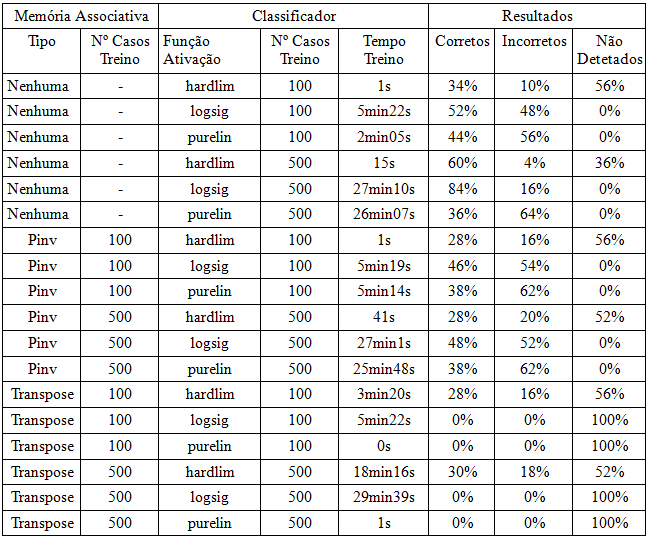
\includegraphics[scale=0.7]{Results.png}
  \caption{Resultados dos testes realizados}
\end{figure}


\pagebreak

\section{Conclusões}

Após uma análise crítica dos resultados obtidos existem alguns pontos que consideramos importante salientar.

O primeiro, e talvez o mais surpreendente, ponto refere-se às arquiteturas implementadas e em comparação neste trabalho: \emph{memória associativa + classificador} vs \emph{classificador}. Analisando os resultados obtidos podemos concluir que a arquitetura que apresenta melhores resultados é a que apenas contém o \emph{classificador}.

De facto, considerámos a \emph{memória associativa} como uma espécie de \emph{"corretor"} dos dados de entrada do sistema, aproximando-os dos respetivos valores perfeitos, o que prevíamos que tornasse a sua classificação mais fácil. No entanto tal não se verificou.

Após analisar o resultado da aplicação de ambas as versões da memória associativa a algumas entradas fornecidas ao sistema, verificámos que este se afastava do valor perfeito respetivo. Mais ainda, este desvio era mais significativo quando os pesos da \emph{memória associativa} eram calculados de acordo com a expressão $target\times input^T$ (já referida neste documento).

Uma possível explicação para este resultado prende-se com o facto da \emph{memória associativa} simular um \emph{"conjunto"} de neurónios, onde se um dado neurónio é ativado, então é bastante provável que os neurónios próximos desse também sejam ativados. Assim, existe uma maior possibilidade de uma dada entrada ser classificada em várias \emph{classes} em simultâneo, e por isso inconclusivas. Desta forma podemos justificar as elevadas percentagens de dados não detetados sempre que utilizámos a \emph{memória associativa}.

%2º ponto --> Aproveitar o facto de estar a falar da MA para introduzir a parte da regra de Hebb e dizer que alternativamente poderiamos implementar uma rede neuronal na MA e fazer um treino iterativo para ela (tal como no classificador), em vez de fazermos um treino em batch, como neste caso.
%3º ponto --> Falar do impacto da dimensão dos dados de trenio na classificação
%4º ponto --> Falar da melhor função de ativação
%5º ponto --> Sistema é capaz de identificar dígitos? Sistema é robusto? Tem boa capacidade de generalização? --> Falar do \textbf que está na linha abaixo desta

\textbf{Referir que os dígitos perfeitos são bem classificados, uma vez que foram incluídos, embora em número reduzido, nos dados de teste da \emph{memória associativa} e do \emph{classificador}. Referir também que alguns dígitos não perfeitos são corretamente classificados.}


\vspace{.3cm}

\textbf{FIXME: Perguntas relatório:}

\begin{itemize}
\item \textbf{How does the data set influence the performance of the classification system?} -- Obtemos melhores resultados (maior número de casos corretamente detetados) quando são utilizados mais casos de teste. Está de acordo com o esperado, uma vez que ao treinarmos o \emph{classificador} com um maior número de exemplos de teste, desde que esse número não seja excessivamente elevado, este vai cobrir um maior número de situações, apresentando uma maior convergência, que resulta numa melhor performance. Quando o número de exemplos de teste é muito elevado, o sistema apresenta uma excelente \emph{performance} para os exemplos de teste, mas uma \emph{performance} inferior para novos exemplos, não contemplados nesses exemplos de teste.

\item Which architecture provides better results: only the classifier or the associative memory+classifier? -- Analisando os resultados obtidos concluímos que a arquitetura que apresenta melhores resultados é, sem dúvida, a arquitetura onde apenas se encontra presente o \emph{classificador}. Uma explicação para este resultado prende-se com o facto da \emph{memória associativa} simular um \emph{"conjunto"} de neurónios, onde se um dado neurónio é ativado, então é bastante provável que os neurónios que o rodeiem também sejam ativados. Com este fenómeno existe uma maior possibilidade de uma dada entrada ser classificada em várias \emph{classes} em simultâneo, justificando as elevadas percentagens de dados não detetados, nos testes realizados com a arquitetura \emph{memória associativa + classificador}.

\item \textbf{Which is the best activation function: hardlim, linear or logsig?} -- Considerando apenas os testes onde obtivemos melhores resultados, isto é, os testes onde não foi utilizada \emph{memória associativa}, a função de ativação que apresentou melhores resultados foi, sem dúvida, a função \emph{sigmoidal, logsig}, uma vez que com essa função obtiveram-se as maiores percentagens de classificações corretas, nomeadamente a maior percentagem de classificações corretas registada em todos os testes realizados: 84\%.

\item \textbf{Does the Hebb rule perform well?} -- Dizer que não aplicámos a regra de Hebb, uma vez que esta só pode ser aplicada para matrizes ortonormadas, o que nem sempre se verifica no nosso caso, dado que o utilizador é livre de desenhar qualquer conjunto de caracteres (que podem não produzir matrizes ortonormadas)

\item \textbf{Is the classification system able to achieve the main objectives (classification of digits)?}

\item \textbf{How is the generalization capacity? Is the classification system robust enough to give correct outputs when new inputs are not perfect? Which is the percentage of well classified new inputs?}
\end{itemize}

\textbf{Fazer pequeno resumo!}

\pagebreak

\section{Anexos}

\begin{figure}[h]
  \centering
      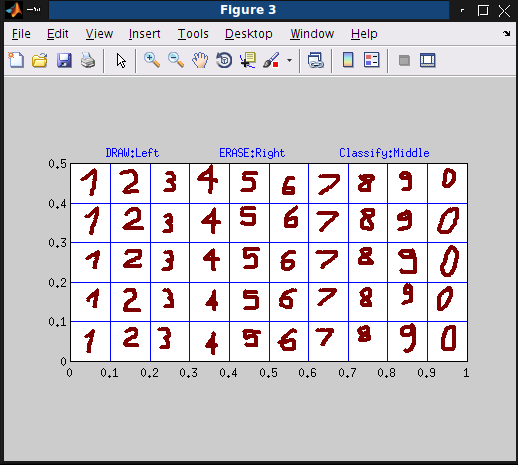
\includegraphics[scale=0.3]{Input.png}
  \caption{Dados de entrada utilizados para os testes realizados à aplicação}
\end{figure}

\begin{figure}[h]
  \centering
      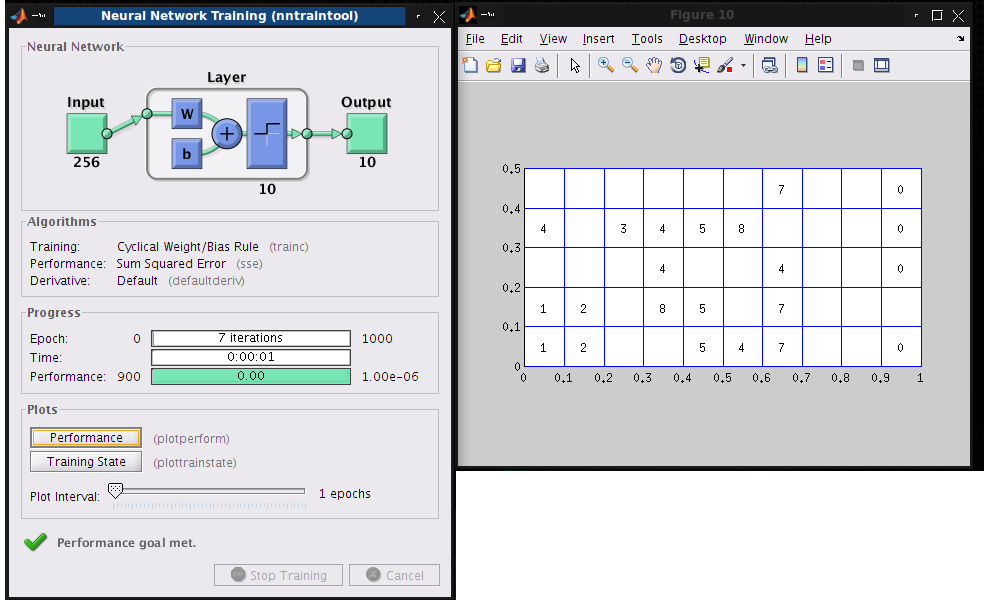
\includegraphics[scale=0.3]{100_Hardlim.png}
  \caption{Tempo de treino da rede neuronal do classificador recorrendo a dados de treino com 100 elementos, utilizando a função \emph{hardlim} como função de ativação e sem utilização de \emph{memória associativa}. São também visíveis os resultados da classificação do input da figura 3}
\end{figure}

\begin{figure}[h]
  \centering
      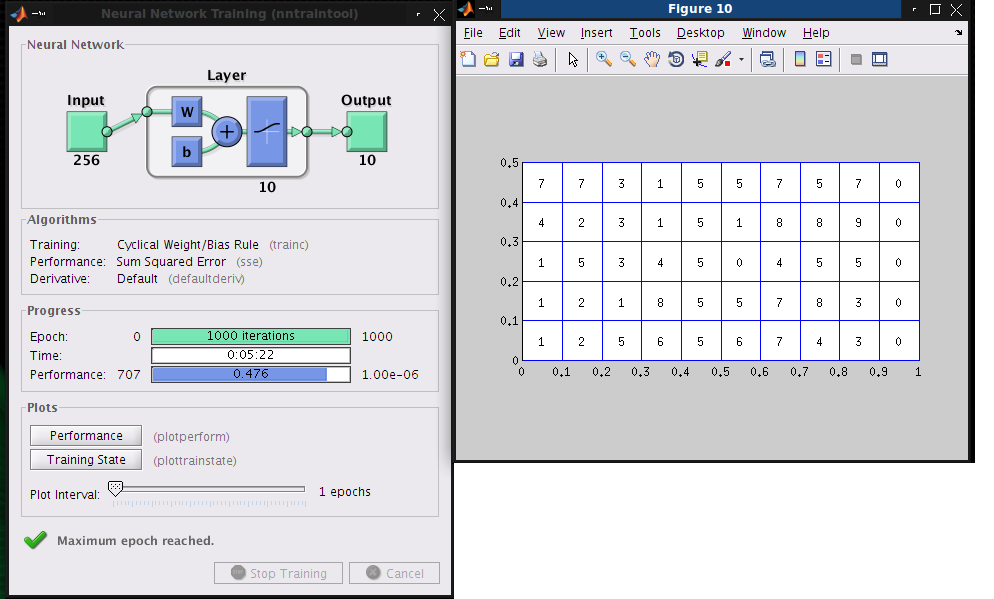
\includegraphics[scale=0.3]{100_Sigmoidal.png}
  \caption{Tempo de treino da rede neuronal do classificador recorrendo a dados de treino com 100 elementos, utilizando a função \emph{logsig} como função de ativação e sem utilização de \emph{memória associativa}. São também visíveis os resultados da classificação do input da figura 3}
\end{figure}

\begin{figure}[h]
  \centering
      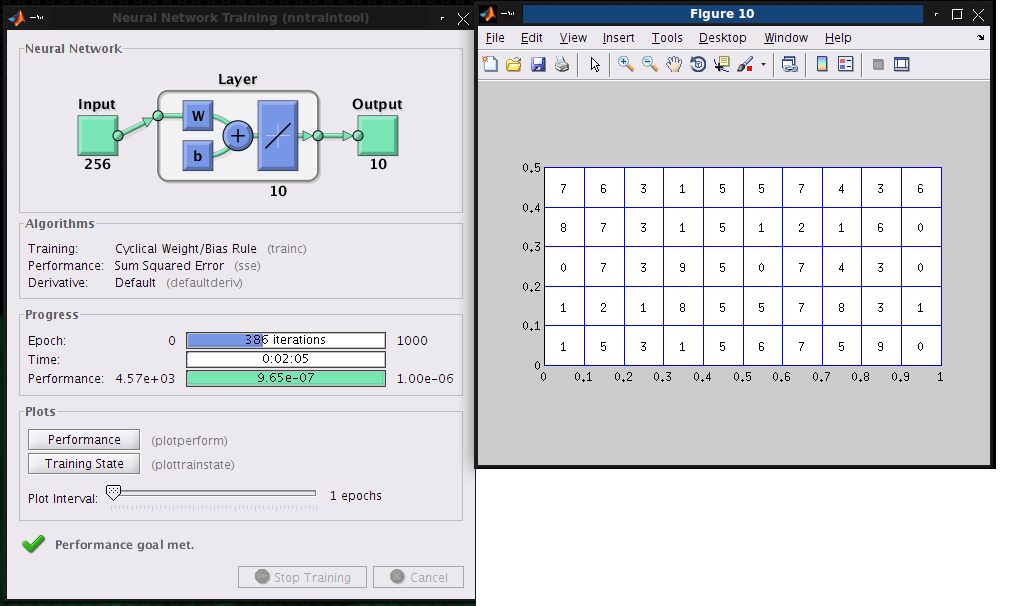
\includegraphics[scale=0.3]{100_Linear.png}
  \caption{Tempo de treino da rede neuronal do classificador recorrendo a dados de treino com 100 elementos, utilizando a função \emph{purelin} como função de ativação e sem utilização de \emph{memória associativa}. São também visíveis os resultados da classificação do input da figura 3}
\end{figure}

\begin{figure}[h]
  \centering
      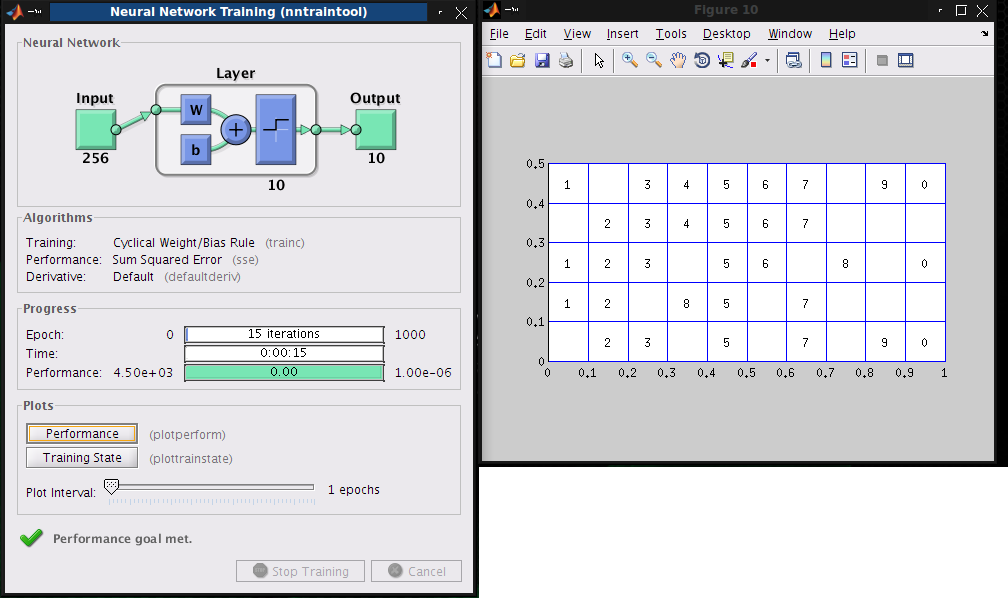
\includegraphics[scale=0.3]{500_Hardlim.png}
  \caption{Tempo de treino da rede neuronal do classificador recorrendo a dados de treino com 500 elementos, utilizando a função \emph{hardlim} como função de ativação e sem utilização de \emph{memória associativa}. São também visíveis os resultados da classificação do input da figura 3}
\end{figure}

\begin{figure}[h]
  \centering
      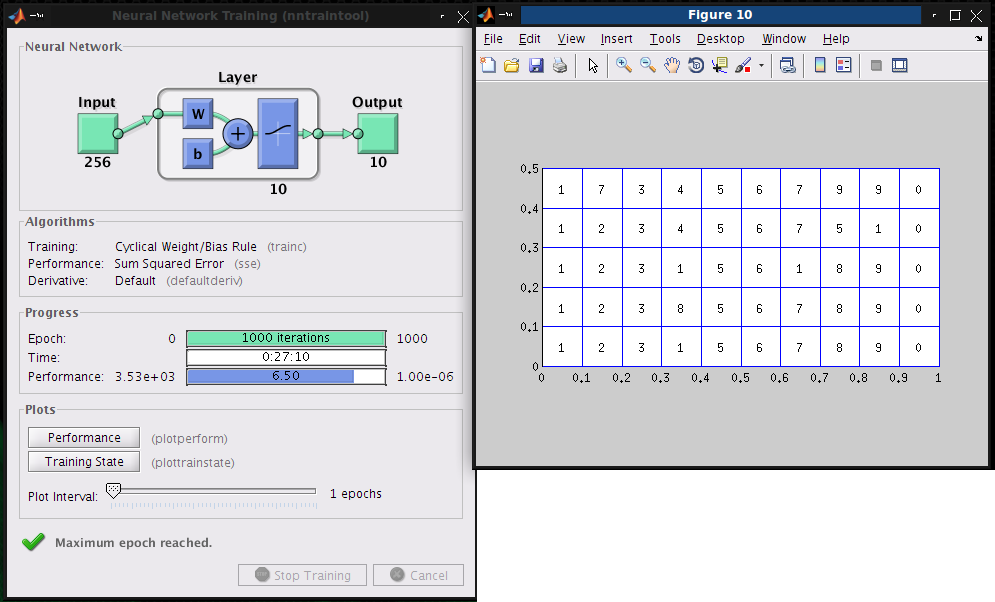
\includegraphics[scale=0.3]{500_Sigmoidal.png}
  \caption{Tempo de treino da rede neuronal do classificador recorrendo a dados de treino com 500 elementos, utilizando a função \emph{logsig} como função de ativação e sem utilização de \emph{memória associativa}. São também visíveis os resultados da classificação do input da figura 3}
\end{figure}

\begin{figure}[h]
  \centering
      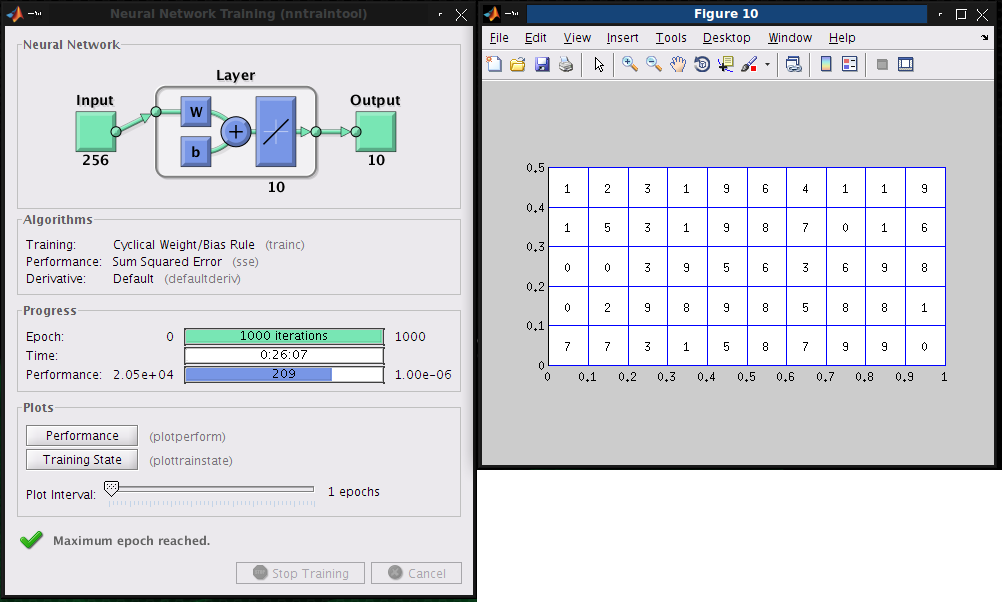
\includegraphics[scale=0.3]{500_Linear.png}
  \caption{Tempo de treino da rede neuronal do classificador recorrendo a dados de treino com 500 elementos, utilizando a função \emph{purelin} como função de ativação e sem utilização de \emph{memória associativa}. São também visíveis os resultados da classificação do input da figura 3}
\end{figure}

\begin{figure}[h]
  \centering
      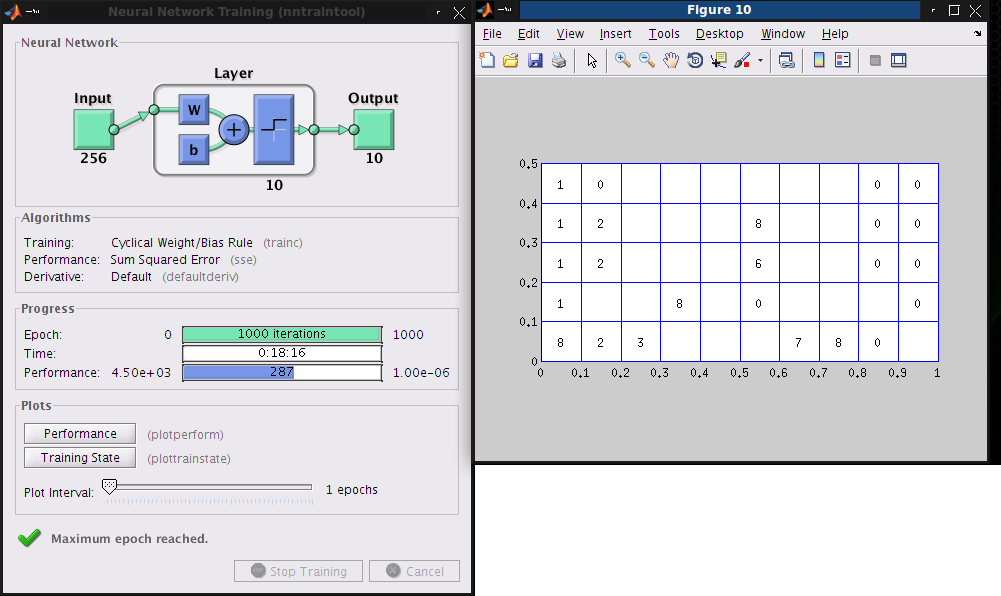
\includegraphics[scale=0.3]{500_Transpose_Hardlim.png}
  \caption{Tempo de treino da rede neuronal do classificador recorrendo a dados de treino com 500 elementos, utilizando a função \emph{hardlim} como função de ativação e com utilização de \emph{memória associativa}, fazendo uso da fórmula $target\times input^T$. São também visíveis os resultados da classificação do input da figura 3}
\end{figure}

\begin{figure}[h]
  \centering
      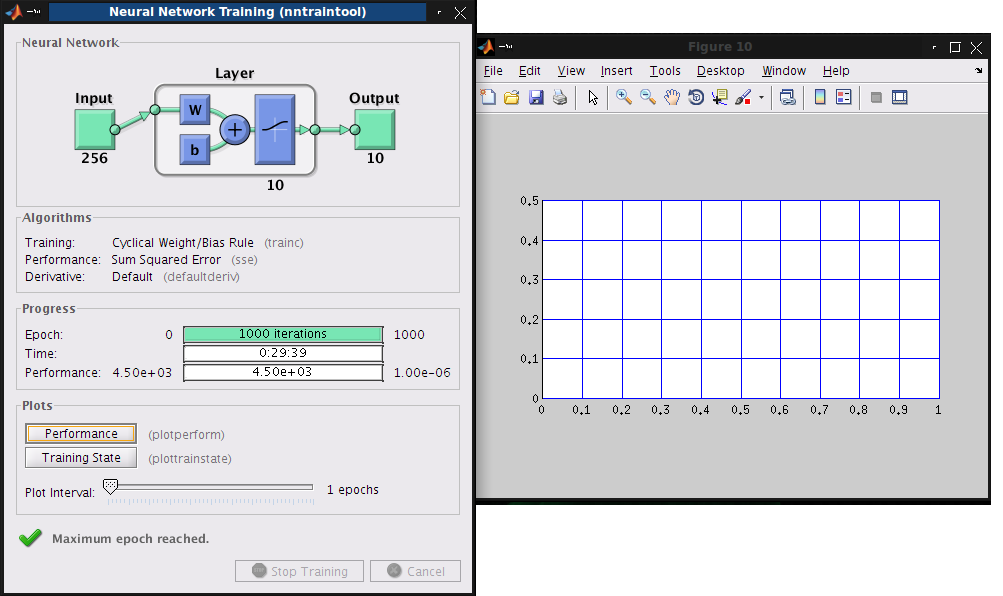
\includegraphics[scale=0.3]{500_Transpose_Sigmoidal.png}
  \caption{Tempo de treino da rede neuronal do classificador recorrendo a dados de treino com 500 elementos, utilizando a função \emph{logsig} como função de ativação e com utilização de \emph{memória associativa}, fazendo uso da fórmula $target\times input^T$. São também visíveis os resultados da classificação do input da figura 3}
\end{figure}

\begin{figure}[h]
  \centering
      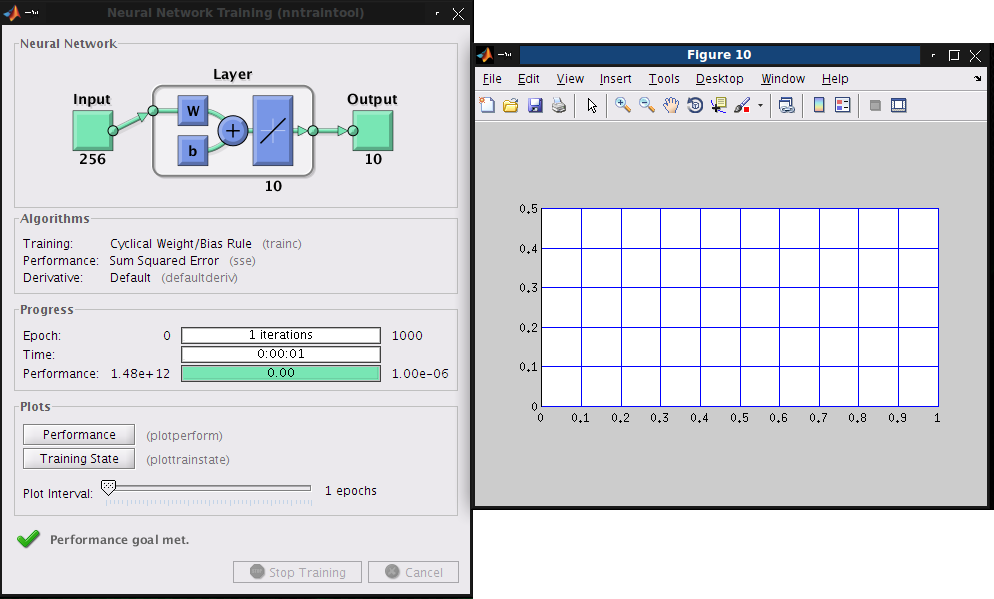
\includegraphics[scale=0.3]{500_Transpose_Linear.png}
  \caption{Tempo de treino da rede neuronal do classificador recorrendo a dados de treino com 500 elementos, utilizando a função \emph{purelin} como função de ativação e com utilização de \emph{memória associativa}, fazendo uso da fórmula $target\times input^T$. São também visíveis os resultados da classificação do input da figura 3}
\end{figure}

\begin{figure}[h]
  \centering
      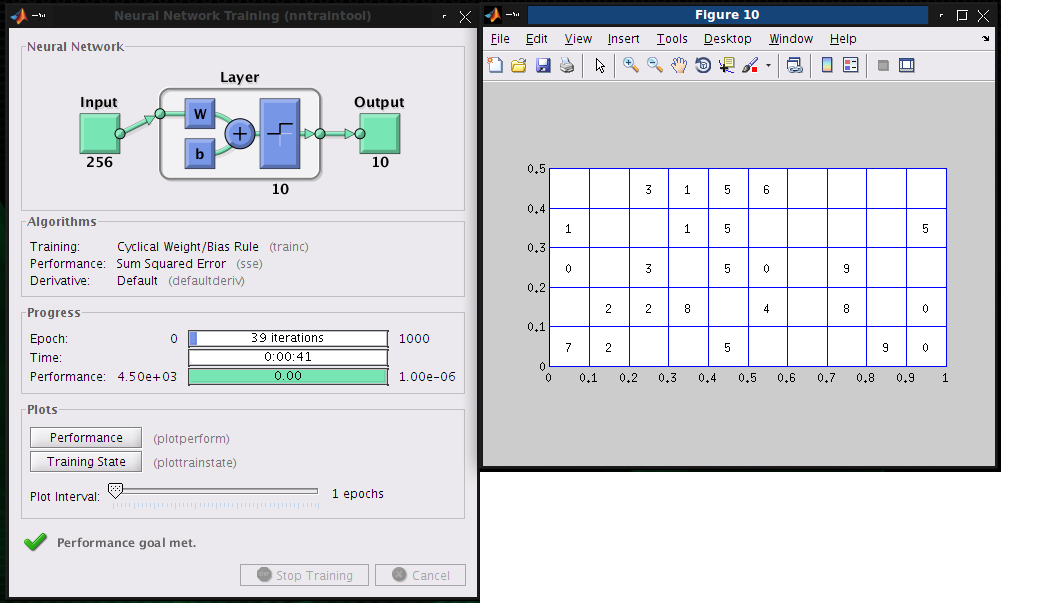
\includegraphics[scale=0.3]{500_Pinv_Hardlim.png}
  \caption{Tempo de treino da rede neuronal do classificador recorrendo a dados de treino com 500 elementos, utilizando a função \emph{hardlim} como função de ativação e com utilização de \emph{memória associativa}, fazendo uso da fórmula $target\times pinv(input)$. São também visíveis os resultados da classificação do input da figura 3}
\end{figure}

\begin{figure}[h]
  \centering
      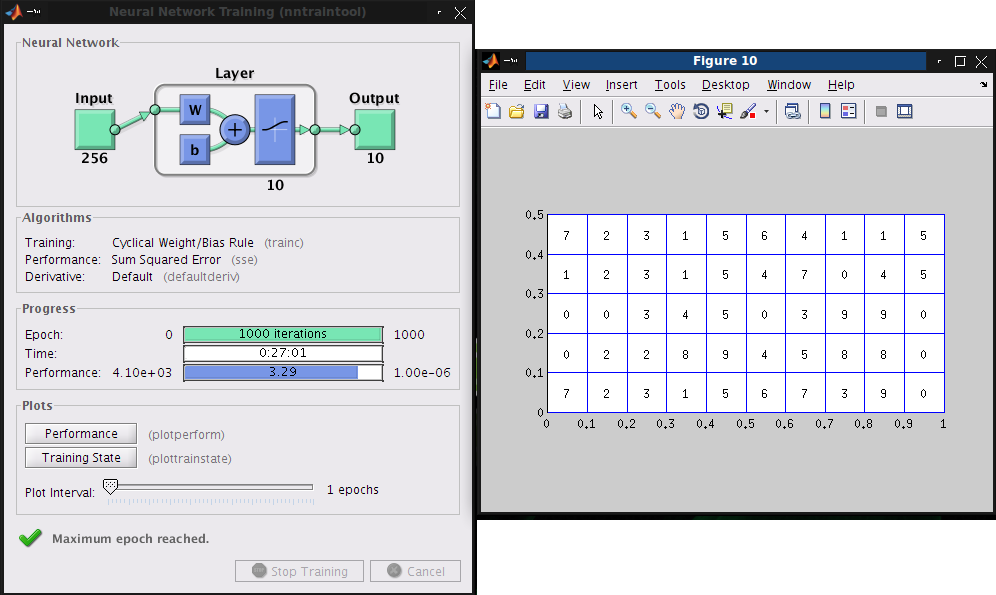
\includegraphics[scale=0.3]{500_Pinv_Sigmoidal.png}
  \caption{Tempo de treino da rede neuronal do classificador recorrendo a dados de treino com 500 elementos, utilizando a função \emph{logsig} como função de ativação e com utilização de \emph{memória associativa}, fazendo uso da fórmula $target\times pinv(input)$. São também visíveis os resultados da classificação do input da figura 3}
\end{figure}

\begin{figure}[h]
  \centering
      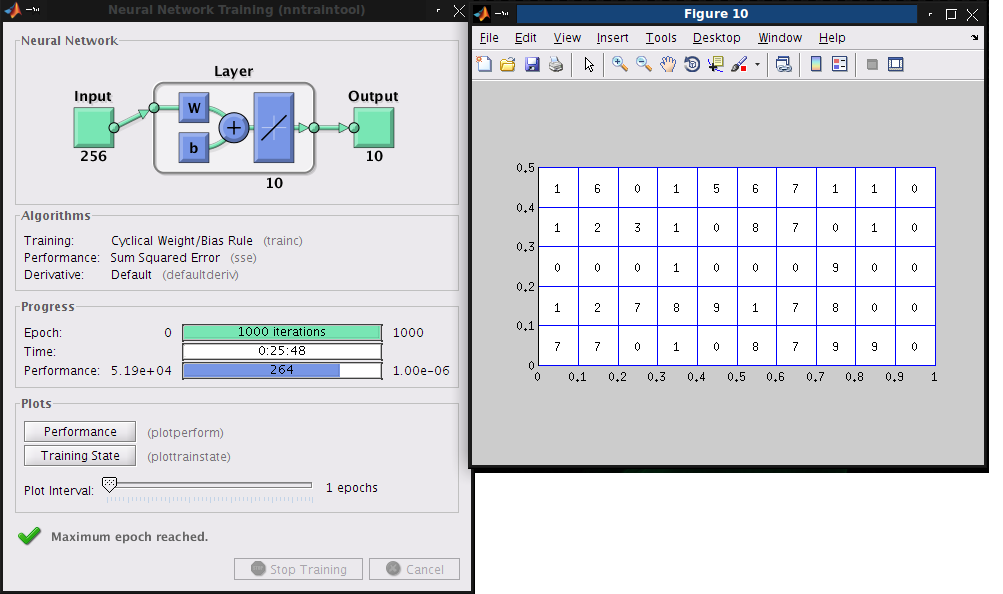
\includegraphics[scale=0.3]{500_Pinv_Linear.png}
  \caption{Tempo de treino da rede neuronal do classificador recorrendo a dados de treino com 500 elementos, utilizando a função \emph{purelin} como função de ativação e com utilização de \emph{memória associativa}, fazendo uso da fórmula $target\times pinv(input)$. São também visíveis os resultados da classificação do input da figura 3}
\end{figure}


\begin{figure}[h]
  \centering
      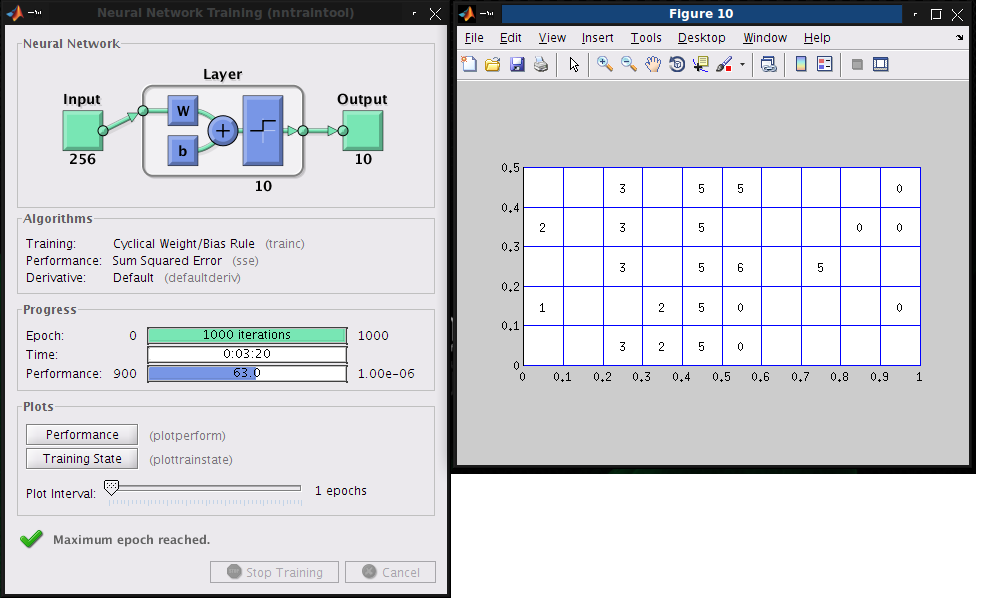
\includegraphics[scale=0.3]{100_Transpose_Hadlim.png}
  \caption{Tempo de treino da rede neuronal do classificador recorrendo a dados de treino com 100 elementos, utilizando a função \emph{hardlim} como função de ativação e com utilização de \emph{memória associativa}, fazendo uso da fórmula $target\times input^T$. São também visíveis os resultados da classificação do input da figura 3}
\end{figure}

\begin{figure}[h]
  \centering
      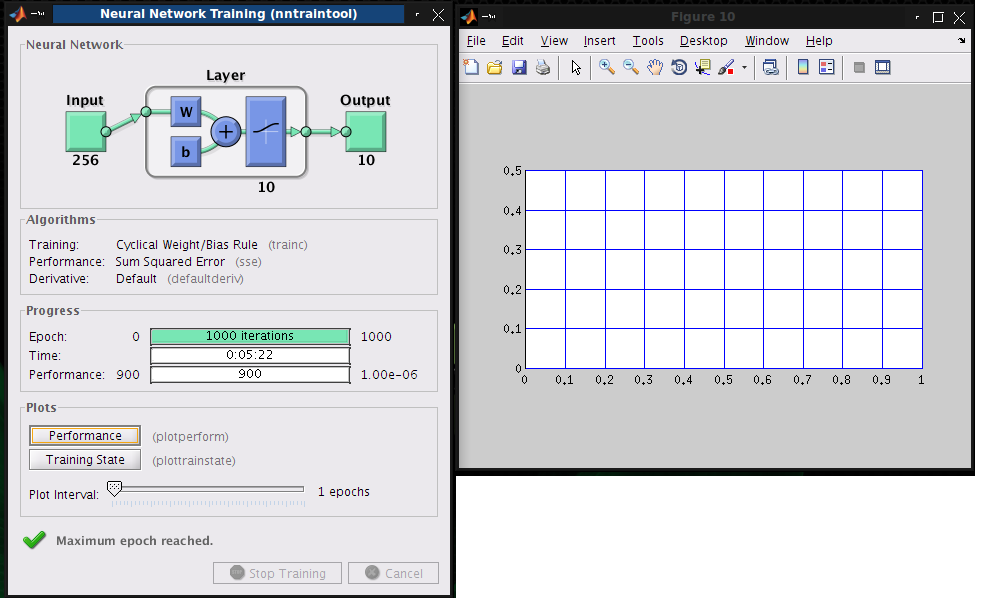
\includegraphics[scale=0.3]{100_Transpose_Sigmoidal.png}
  \caption{Tempo de treino da rede neuronal do classificador recorrendo a dados de treino com 100 elementos, utilizando a função \emph{logsig} como função de ativação e com utilização de \emph{memória associativa}, fazendo uso da fórmula $target\times input^T$. São também visíveis os resultados da classificação do input da figura 3}
\end{figure}

\begin{figure}[h]
  \centering
      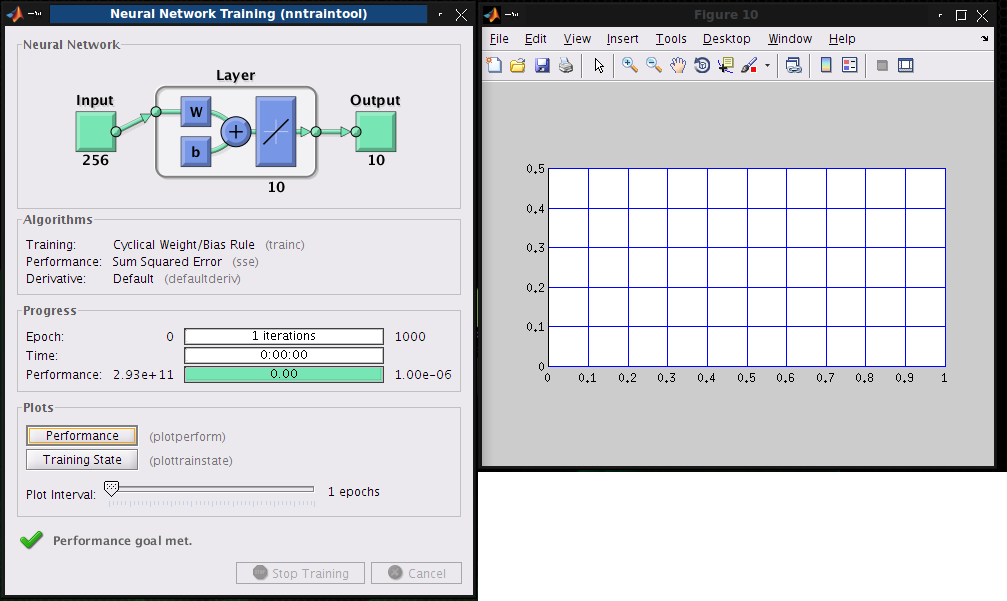
\includegraphics[scale=0.3]{100_Transpose_Linear.png}
  \caption{Tempo de treino da rede neuronal do classificador recorrendo a dados de treino com 100 elementos, utilizando a função \emph{purelin} como função de ativação e com utilização de \emph{memória associativa}, fazendo uso da fórmula $target\times input^T$. São também visíveis os resultados da classificação do input da figura 3}
\end{figure}

\begin{figure}[h]
  \centering
      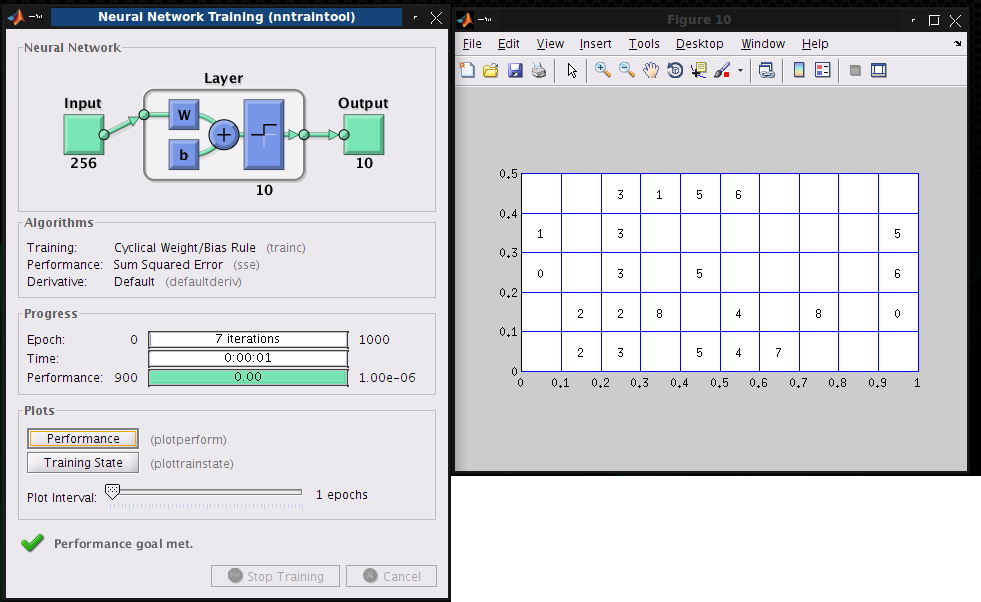
\includegraphics[scale=0.3]{100_Pinv_Hardlim.png}
  \caption{Tempo de treino da rede neuronal do classificador recorrendo a dados de treino com 100 elementos, utilizando a função \emph{hardlim} como função de ativação e com utilização de \emph{memória associativa}, fazendo uso da fórmula $target\times pinv(input)$. São também visíveis os resultados da classificação do input da figura 3}
\end{figure}

\begin{figure}[h]
  \centering
      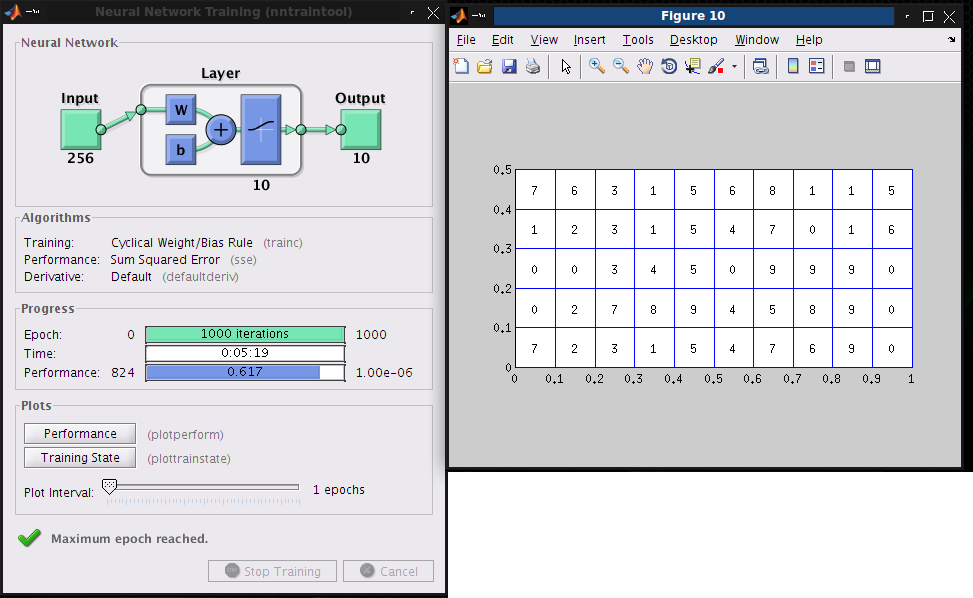
\includegraphics[scale=0.3]{100_Pinv_Sigmoidal.png}
  \caption{Tempo de treino da rede neuronal do classificador recorrendo a dados de treino com 100 elementos, utilizando a função \emph{logsig} como função de ativação e com utilização de \emph{memória associativa}, fazendo uso da fórmula $target\times pinv(input)$. São também visíveis os resultados da classificação do input da figura 3}
\end{figure}

\clearpage

\begin{figure}[h]
  \centering
      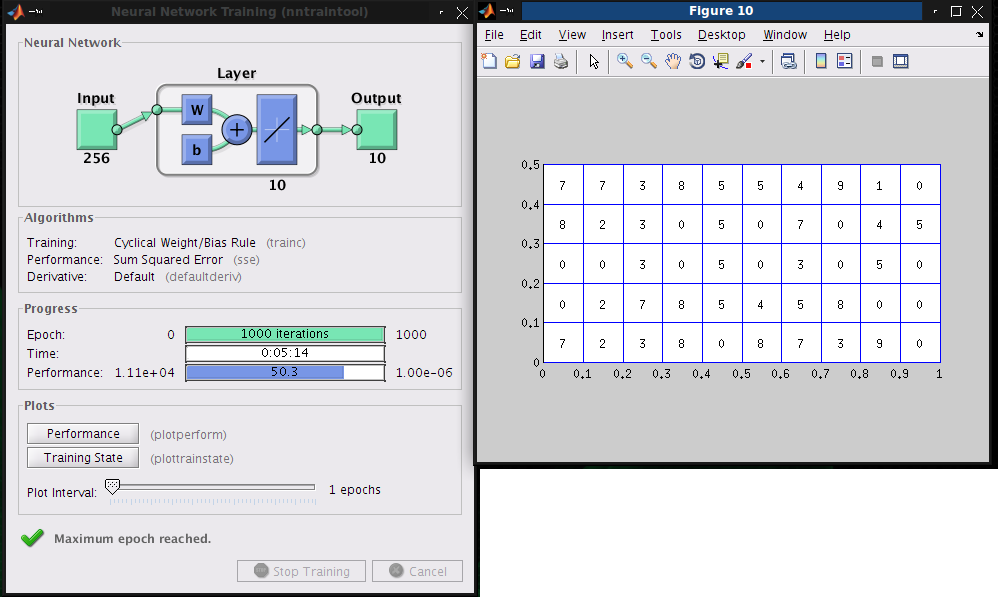
\includegraphics[scale=0.3]{100_Pinv_Linear.png}
  \caption{Tempo de treino da rede neuronal do classificador recorrendo a dados de treino com 100 elementos, utilizando a função \emph{purelin} como função de ativação e com utilização de \emph{memória associativa}, fazendo uso da fórmula $target\times pinv(input)$. São também visíveis os resultados da classificação do input da figura 3}
\end{figure}

\end{document}